\documentclass{article}

\usepackage[%
    left=0.5in,%
    right=0.5in,%
    top=0.5in,%
    bottom=0.5in,%
]{geometry}%
\usepackage{minitoc}
\usepackage{multicol}
\usepackage{graphicx}
\usepackage{fixltx2e}
\usepackage{listings}
\usepackage{color}
\usepackage{hyperref}
    \hypersetup{ colorlinks = true, linkcolor = blue }
\usepackage{blindtext}
\definecolor{lightgray}{gray}{0.9}
\graphicspath{ {./} }

\newcommand{\inlinecode}[2]{\colorbox{lightgray}{\lstinline
[language=#1]$#2$}}
\newcommand{\worddef}[1]{\hyperref[sec:reference]{\textit{#1}}}

\begin{document}

\tableofcontents

\newpage

\section{Architecture}

\begin{multicols}{2}
\begin{itemize}
  \item A software stack for mobile devices
  \item Operating system kernel
  \item Standard middleware
  \begin{itemize}
    \item Android library support
  \end{itemize}
  \item Key applications / user interfaces
  \begin{itemize}
    \item Vendor specific modifications
  \end{itemize}
  \item LK: threading, low level memory management, driver
  \item HAL: libs for hardware module
  \item AR: virtual machine
  \item NCL: fundamental core functionalities
  \item API: programming interface
  \item APP: system apps can be customised.
\end{itemize}

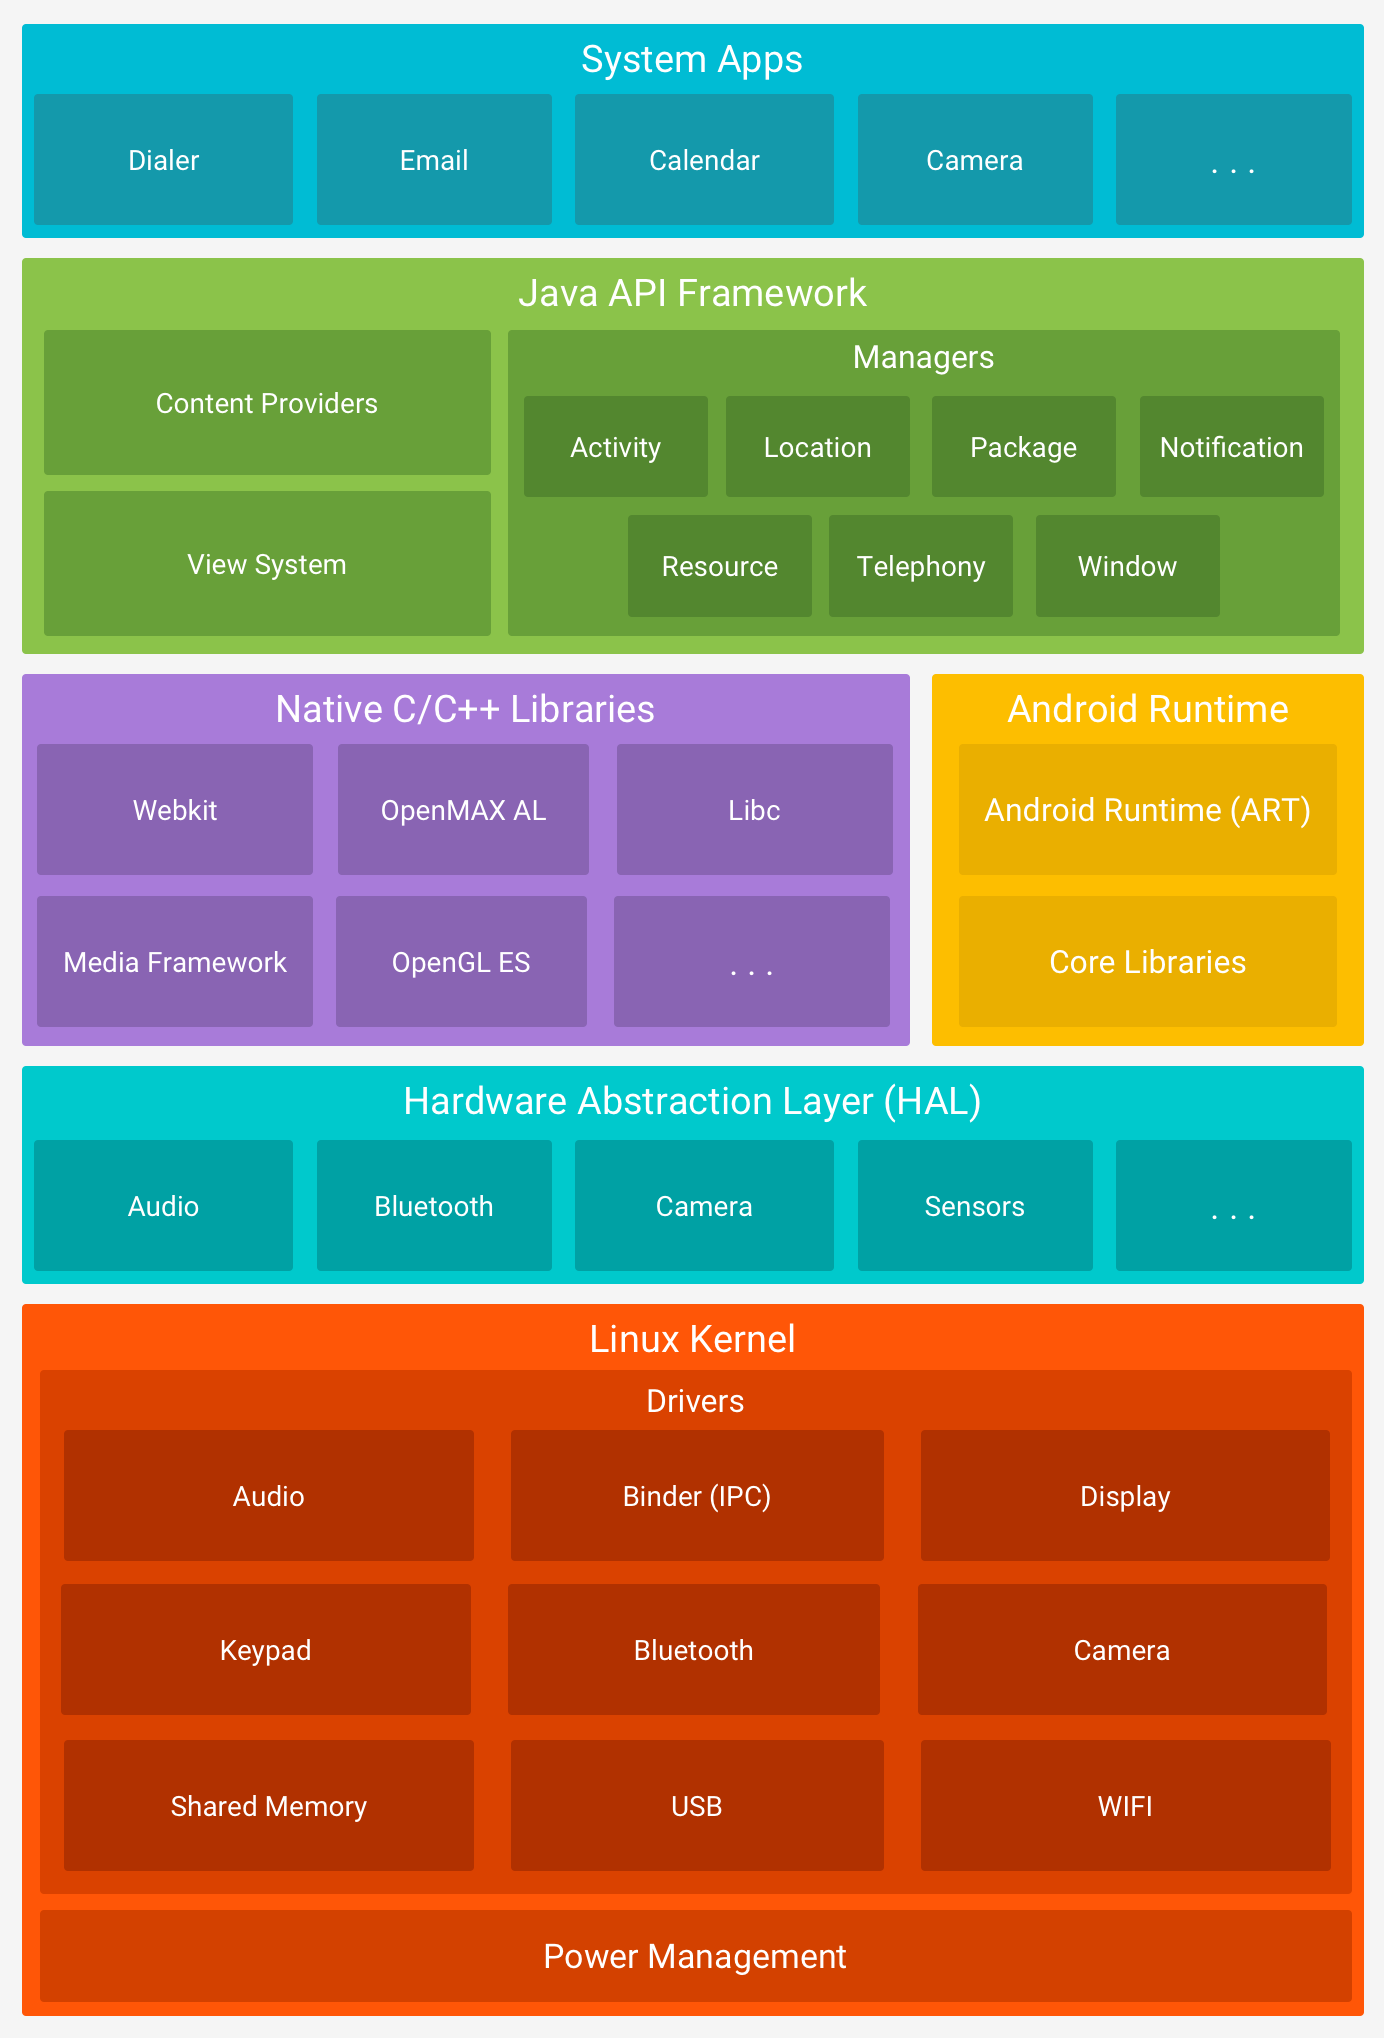
\includegraphics[scale=0.1]{android-stack_2x.png}

\end{multicols}

\subsection{Kernel}

\begin{multicols}{2}

\subsubsection{Modifications}

\begin{flushleft}
  Modifications made by android to linux OS
\end{flushleft}
\begin{itemize}
  \item wakelocks
  \begin{itemize}
  	\item Keep the phone awake
  \end{itemize}
  \item binder
  	\begin{itemize}
  		\item Interprocess communication mechanism, and remote method invocation system.
  		\item One Android process can call a routine in another Android process
  	\end{itemize}
  \item ashmem
  \begin{itemize}
  	\item Android Shared Memory
  	\item A component of the Android operating system that facilitates memory sharing and conservation
  \end{itemize}
  \item LMK – kills processes when memory is low
  \item alarm manager
  \begin{itemize}
  	\item Wakes up the phone when necessary
  \end{itemize}
\end{itemize}

\vfill\null

\subsection{Hardware support}
\begin{itemize}
  \item Bluetooth - BlueZ
  \item GPS – Manufacturer provided libgps
  \item Wifi – \texttt{wpa-supplicant}
  \item Display – Standard framebuffer driver
  \item Keyboard – Standard input event
  \item Lights – Manufacturer provided liblights.so
  \item Audio – Manufacturer provided libaudio.so
  \item Camera – Manufacturer provided libcamera.so
  \item Power Management – “wakelocks” kernel patch
  \item Sensors – Manufacturer provided libsensors.so
  \item Radio – Manufacturer provided libril.so
\end{itemize}

\end{multicols}

\subsection{Security}

Applications are sandboxed
\begin{itemize}
 \item A security mechanism for separating running applications and data
 \item This allows applications run in a different context, so if one app crashed, others can stay uneffected
 \item On Android, each app runs as its own \textbf{user}, which guarantees that different users are unable to interfere with each other, access each other’s files and so on. Root can access the entire system
 \item Own process, own VM, own UID/AID for different app
\end{itemize}

\newpage

\section{System boot process}

\begin{multicols}{2}
  \begin{itemize}
		\item \textbf{Boot ROM/ Bootloader:} Load bootloader into RAM, detect external RAM, setup network, memory, etc.
		\item \textbf{Kernel:} Setup cache, protected memory, scheduling and loads drivers.
		\item \textbf{Init:} Mounts directories like /sys , /dev or /proc Runs init.rc script
		\item \textbf{Zygote \& VM:} Enables code sharing across the android VM for quick start of separate VM for different apps preloadClasses(), preloadResources()
		\item \textbf{System service:} Power manager, activity manager, telephony registry, package manger, context manager, system contact providers, etc.
	\end{itemize}
	\vfill\null

	\begin{center}
	  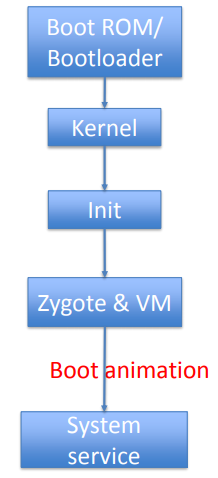
\includegraphics[scale=0.5]{boot_process.png}
	\end{center}
\end{multicols}

\section{Zygote}
\begin{itemize}
  \item Initialised process that has all core libraries linked in
  \item Load all java.*, android.* classes at boot time
  \item Initially create a single android VM process – Referencing classes loaded above
  \item When user runs an application:
  \begin{itemize}
    \item Creates a copy of itself in a separate address space
    \item \textbf{Does not} copy memory, instead refers to original memory until modified
    \item Because each container recieves a map, these resources are shared between applications, eliminating the need for each new fork of the VM to keep its own copy of classes and resource.
  \end{itemize}
\end{itemize}

\section{Memory}
\begin{flushleft}
In many places, Android shares the same dynamic RAM across processes using explicitly allocated shared memory regions.
Android uses paging and mmap instead of providing swap space, which means any memory your application touches cannot be paged out unless you release all references.
\end{flushleft}

\section{Android compilation}

\begin{multicols}{2}
  \begin{itemize}
    \item Applications are written in Java
    \begin{itemize}
      \item Run on Google’s own VM — Dalvik/ Android Run Time
      \item Uses its own bytecode (DEX) format
    \end{itemize}
    \item Code compiled using standard Java tools then convert to DEX format
    \begin{itemize}
      \item Multiple class files can be put in to a single .dex file.
    \end{itemize}
    \item Code, data and resource files packed into a .apk file
  \end{itemize}

  \vfill\null

  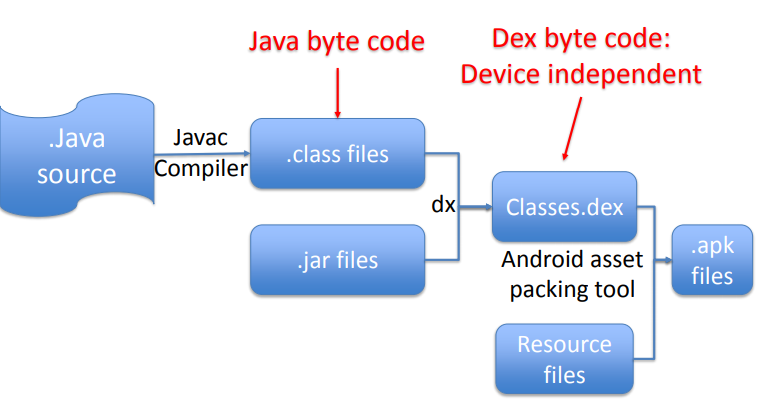
\includegraphics[scale=0.3]{compilation.png}
\end{multicols}

\subsection{Dalvik}

\begin{itemize}
  \item Dalvik architecture is \textit{register based} rather than \textit{stack based}, which make's it optimised to use less space
  \item Execute its own Dalvik byte code rather than Java bytecode
  \item Dalvik interprets .dex files
  \begin{itemize}
    \item Post-processes .class files
    \item Size reduction
    \item JIT compilation to native ARM instructions
  \end{itemize}
  \item Target slow cpu, no swap, low RAM, battery powered device.
  \item This approach allows us to execute less instructions, but the instructions are larger
\end{itemize}

\begin{center}
  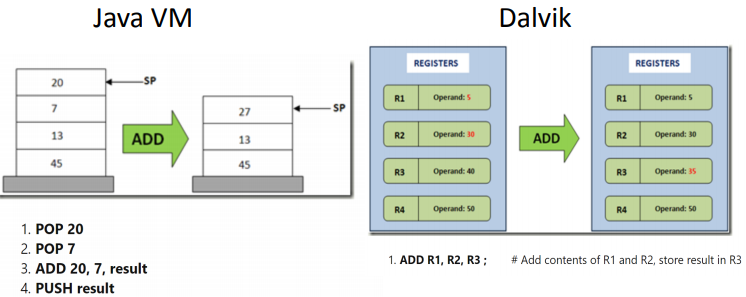
\includegraphics[scale=0.6]{stack_vs_register.png}
\end{center}

\section{Runtime}

\begin{multicols}{2}
  \subsection{Darvik runtime}
  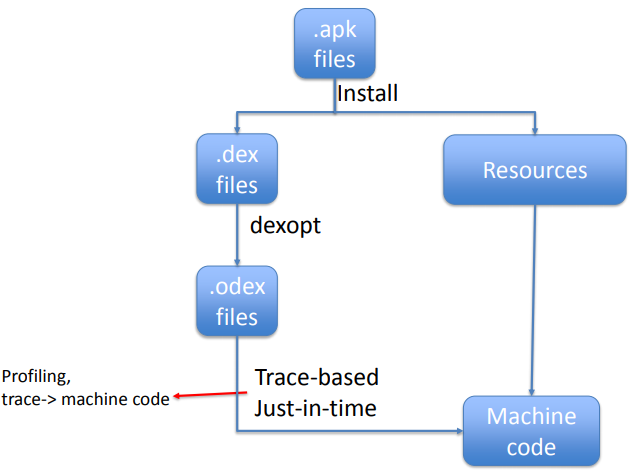
\includegraphics[scale=0.4]{darvik_runtime.png}

  \vfill\null
  
  \subsection{ART runtime}
  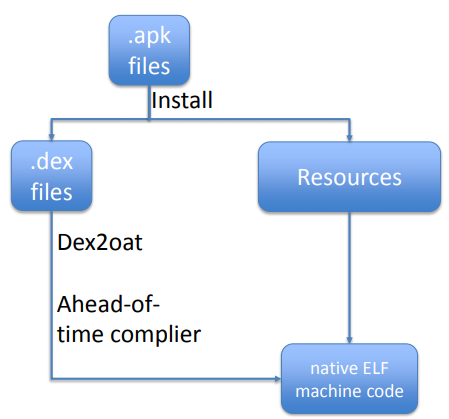
\includegraphics[scale=0.4]{art_runtime.png}
\end{multicols}

\pagebreak

\section{ART}

\begin{itemize}
  \item \textbf{Pros}
  \begin{itemize}
    \item Apps run faster as DEX bytecode translation done during installation
    \item Reduces start-up time of applications as native code is directly executed
    \item Improves battery performance as power utilised to interpreted byte codes line by line is saved
  \end{itemize}
  \item \textbf{Cons}
  \begin{itemize}
    \item App Installation takes more time because of DEX bytecodes conversion into machine code
    \item More internal storage is required to store the fully converted machine code at installation
  \end{itemize}
\end{itemize}

\subsection{Android 7.0}
\begin{flushleft}
Android 7.0 adds a JIT compiler with code profiling to ART that constantly improves the performance of Android apps as they run
\end{flushleft}

\subsection{Programming Models}

\begin{multicols}{2}

\subsection{Comparison}

\begin{flushleft}
Traditional OS applications:
\begin{itemize}
  \item A single entry point
  \item Main – OS loads the program into a process and executes it
\end{itemize}
Java applications:
\begin{itemize}
  \item A Java VM is instantiated
  \item Loads all classes used by the application
  \item Executes main
\end{itemize}
Component based model
\begin{itemize}
  \item Multiple application entry points
  \item The point through which the system can “enter” the application
\end{itemize}
\end{flushleft}

\smallskip
\subsection{Android components}

Activities
\begin{itemize}
  \item Dictate the UI and handle the user interaction to the smart phone screen.
\end{itemize}
Services
\begin{itemize}
  \item Mechanism for doing something long-running in the
background
  \item Handle background processing associated with an application.
\end{itemize}
Broadcast Receivers
\begin{itemize}
  \item Respond to broadcast messages from the OS / other
apps
\end{itemize}
Content Providers
\begin{itemize}
  \item Make data available to / make use of data from other
apps
\end{itemize}

\end{multicols}

\newpage

\begin{description}
	\item[placeholder] \hfill \\
\end{description}
\end{document}
